
\chapter{Implementierung}
\label{implementierung}

\paragraph{} In diesem Kapitel ist die Umsetzung der in Kapitel \ref{methoden} vorgestellten Konzepte und Methoden beschrieben. Das schließt sowohl die Architektur der Implementierung (siehe \ref{impl-architecture}) als auch eine detaillierte Beschreibung der Algorithmen ein, wie sie im fertigen Programm vorliegen (siehe \ref{impl-algorithms}).

\section{Systemarchitektur}
\label{impl-architecture}

\paragraph{} Die fertige Systemarchitektur entspricht weitgehend dem vorgeschlagenen Konzept (siehe Anhang \ref{uml-architecture}). Das System gliedert sich vornehmlich in folgende Bereiche:
\begin{enumerate}
\item Das Hauptpaket liefert die API für alle Anfragen an das Programm und leistet den Import von Dokumenten (siehe \ref{arch-import}).
\item Hilfsklassen für das Hauptpaket übernehmen die Einteilung von Suchanfragen in Suchmodi, erledigen exakte Suchanfragen und kümmern sich um die Sortierung aller Suchergebnisse (siehe \ref{arch-helper}).
\item Das Indexpaket bildet Dokumente, Worte und Vorkommen in einer Indexstruktur ab (siehe \ref{arch-index}).
\item Die Worte werden ebenfalls in einem Suffixbaum gespeichert, um damit Suchanfragen in den übrigen Modi zu bearbeiten (siehe \ref{arch-suffix}).
\item Ein Tochterpaket des Suffixbaum-Pakets enthält die Feinumsetzung von Suchanfragen in Semantik und die Unterstützung des eigentlichen Matchings (siehe \ref{arch-pattern}).
\end{enumerate}

\paragraph{} Zusätzlich existieren noch die Pakete \texttt{results}, \texttt{exceptions}, \texttt{util} und \texttt{xmltools} zu Unterstützungszwecken. Im Anhang ist die Paketstruktur auch in einem UML-Paketdiagramm visualisiert (siehe \ref{uml-package}).

\paragraph{} Im Folgenden werden die wichtigsten Pakete und Klassen des Systems beschrieben. Genauere Informationen über die einzelnen Methoden und Attribute sind im JavaDoc\texttrademark des Programms enthalten. Eine grafische Übersicht liefert das Klassendiagramm im Anhang (siehe \ref{uml-classes}).

\subsection{Import und Schnittstelle}
\label{arch-import}

\paragraph{} Für Anfragen von außen steht das Hauptpaket, \texttt{de.unibi.cebitec.bibiserv.\\search} zur Verfügung. Alle Anfragen - Einfügen und Entfernen von Dokumenten in den Suchraum sowie die Suche selbst - können hierüber angestoßen werden. Auch alle Rückgabewerte der entsprechenden Methoden werden in Instanzen dieses Pakets ausgedrückt. Für den Import wird dabei auf das "`Apache Tika"'-Paket\footnote{siehe \url{http://tika.apache.org/}} zurückgegriffen. Damit ist es möglich, alle für den \textit{BiBiServ2} relevanten Dokument-Typen zu bearbeiten (siehe auch \ref{intro-compatibility}).

\subsubsection{Search}
\label{arch-search}

\paragraph{} Mit ihrer Tochterklasse \texttt{BiBiServSearch} bildet \texttt{Search} beinahe die gesamte API der Anwendung. Hierüber werden alle wesentlichen Befehle von außen angestoßen. Die wichtigsten Methoden sind:

\paragraph{getInstance:} Gibt die einzige Instanz der search-Klasse zurück.

\paragraph{addDocuments:} Fügt neue Dokumente in den Suchraum ein (siehe auch \ref{algo-addDoc}).

\paragraph{search:} Stößt eine Suche für das gegebene Suchmuster an und gibt anschließend eine sortierte Liste mit Suchergebnissen zurück. Details dazu sind im Kapitel \ref{impl-algorithms} zu finden.

\paragraph{removeDocument:} Entfernt ein Dokument anhand seiner URL (siehe auch \ref{algo-removeDoc}).

\subsubsection{OutputSearchResult}

\paragraph{} Diese Klasse repräsentiert ein Suchergebnis. Es enthält die URL des Dokuments, in dem das Suchmuster gefunden wurde und eine (unsortierte) Liste von Treffern, die für das Suchmuster im Dokument gefunden wurden. Diese Treffer können Nutzenden dann angezeigt werden (siehe auch Abbildung \ref{fig-matches-screenshot}).

\newpage

\subsection{Hilfsklassen für Suchvorgänge}
\label{arch-helper}

\paragraph{} Im Hintergrund des Hauptpaketes wirken für Vor- und Nachbereitung von Suchanfragen sowie die Bearbeitung der exakten Suche einfache Hilfsklassen. Die wichtigsten davon sind hier vorgestellt.

\subsubsection{SearchQuery}

\paragraph{} Diese Klasse repräsentiert eine Suchanfrage. Sie enthält den Typ der Suchanfrage (Exakte Suche, Teilwortsuche oder Inexakte Suche, siehe auch \ref{anforderungen-features}) sowie die Worte, nach denen gesucht werden soll. Ihre wichtigste Methode ist:

\paragraph{parseQuery:} Mit dieser statischen Methode wird aus einem Eingabestring eine Instanz der \texttt{SearchQuery}-Klasse erzeugt.

\subsubsection{SearchScore}

\paragraph{} Ein \texttt{SearchScore}-Objekt repräsentiert die Wertung eines Suchergebnisses. Die wichtigste Methode hier ist:

\paragraph{calculateScoredResults:} Diese statische Methode sortiert eine Liste von Suchergebnissen nach "`Relevanz"'. Die Details zur Bewertung von Suchergebnissen sind in Kapitel \ref{algo-scoring} beschrieben.

\subsubsection{ExactMatcher}

\paragraph{} Eine \texttt{ExactMatcher}-Instanz kann für ein gegebenes Array von Worten eine exakte Suche durchführen, bei der die Worte in genau dieser Reihenfolge gesucht werden.

\paragraph{getMatches:} Startet den eigentlichen Suchvorgang und gibt etwaige Treffer zurück.

\subsection{Indexstruktur}
\label{arch-index}

\paragraph{} Das in Kapitel \ref{meth-hashing} beschriebene Hashing findet im Paket \texttt{de.unibi.cebitec.\\bibiserv.search.index} statt. Üblicherweise werden dabei Datensätze über eine eindeutige ID referenziert. Dies dient zur Reduzierung des Speicherverbrauchs, weil die IDs eine feste Größe besitzen. Im Einzelnen sind die Schlüssel-Wert-Kombinationen wie folgt:

\paragraph{}

\begin{tabularx}{\textwidth}{llX}
\hline
\textbf{Klasse} & \textbf{Argument-Klasse} & \textbf{Wert-Klasse} \\ [0.1cm]
\hline
MainIndex & WordID & OccurenceSet \\ [0.1cm]
\hline
BiBiServDocument & DocumentID & BiBiServDocument \\ [0.1cm]
\hline
WordIndex & String & WordID \\ [0.1cm]
\hline
\end{tabularx}

\paragraph{} Alle Indizes sind Instanzen der Klasse \texttt{de.unibi.cebitec.bibiserv.search.\\util.Index}. Diese Klasse erweitert allerdings lediglich die übliche \texttt{HashMap} um Synchronisierungsmethoden, um thread-sicheren Zugriff zu ermöglichen. Die Index-Klassen, die hier vorgestellt werden, stellen jeweils nur statische Methoden zur Verfügung, da jeder Index nur einmal im Speicher liegen soll.

\subsubsection{Occurence}

\paragraph{} Diese Klasse implementiert das Vorkommen eines Wortes. Ein Vorkommen referenziert die ID des Wortes, dessen Vorkommen es ist, die ID des Dokuments, in dem es vorkommt, sowie den eigenen Vorgänger und Nachfolger im indizierten Text (Im Text "`der holde Knabe"' wäre der Vorgänger des Vorkommens des Wortes "`holde"' z.B. ein bestimmtes Vorkommen des Wortes "`der"'). Dabei wird die Referenzierung von Vorgängern und Nachfolgern bei Vorkommen sowohl für die exakte Suche benutzt (siehe \ref{algo-exact}) als auch für die Darstellung von Suchergebnissen für Nutzende des Programms: Auf der Ergebnisseite wird nicht nur das Suchergebnis selbst, sondern auch die Umgebung des Treffers angezeigt (siehe Abbildung \ref{fig-matches-screenshot}).

\subsubsection{MainIndex}
\label{arch-mainIndex}

\paragraph{} Der Hauptindex beantwortet die Suchanfragen der Search-Klasse und bildet die IDs von Worten auf eine Menge von Vorkommen dieser Worte ab. Die wesentlichen Funktionen dieser Klasse sind:

\paragraph{indexOccurence:} Indiziert das Vorkommen eines Wortes bei der Neueinfügung eines Dokuments.

\paragraph{searchExactly:} Sucht die Vorkommen eines Wortes in seiner exakten Schreibweise aus dem Index heraus. Die genaue Funktionsweise wird näher in Kapitel \ref{algo-exact} beschrieben.

\paragraph{searchSuperStrings:} Reicht eine Suchanfrage an den Suffixbaum weiter.

\paragraph{getOccurencesForWordID:} Gibt alle Vorkommen eines Wortes mit der gegebenen ID zurück. Dies ist die eigentliche Indexfunktion des Hauptindex und wird bei allen Suchanfragen benutzt.

\paragraph{removeDocumentReferencesByID:} Es werden alle Wortvorkommen aus dem Index entfernt, die zum Dokument mit der gegebenen ID gehören.

\subsubsection{WordIndex}
\label{arch-wordIndex}

\paragraph{} Der Wortindex ist dazu da, sowohl in einem Verzeichnis von Worten als auch im Suffixbaum alle Worte einzufügen, die indiziert werden. Der Index selbst bildet Worte auf ihre jeweilige ID ab. Der umgekehrte Weg (also die Abbildung von Wort-IDs auf Worte) ist ebenfalls an vielen Stellen nötig, wird aber über einen Pointer in den WordIDs selbst erledigt. Die wichtigsten Funktionen dieser Klasse sind:

\paragraph{indexWord:} Fügt ein Wort in den Index ein (sofern es noch nicht indiziert ist) und gibt die (ggf. neu erzeugte) ID des Wortes zurück.

\paragraph{getTreeInstance:} Diese Funktion stellt den Suffixbaum nach außen hin zur Verfügung. Die Bauminstanz wird zum Beispiel vom Hauptindex zur Beantwortung von Suchanfragen benötigt.

\paragraph{getID:} Gibt die ID eines gegeben Wortes zurück oder \texttt{null}, falls das Wort nicht indiziert ist.

\paragraph{removeWord:} Entfernt (mit den beiden Schwesterfunktionen \texttt{removeWordByID} und \texttt{removeWordByReference}) Worte aus dem Index. Das kommt dann vor, wenn Dokumente aus dem Index entfernt werden.

\subsubsection{SuffixTreeAppendSession}
\label{arch-session}

\paragraph{} Diese Klasse ermöglicht das Einfügen von Worten in den Suffixbaum. Das setzt das in Abschnitt \ref{meth-addAndRemove} vorgeschlagene Synchronisationssystem um. Die API-Methoden für eine solche Session sind:

\paragraph{open:} Öffnet eine Session, in der Worte zum Suffixbaum hinzugefügt werden können. Dabei wird aus dem momentanen Wort-Index der aktuelle Suffixbaum als Kopie neu aufgebaut. Es wird auch sichergestellt, dass nur eine Session gleichzeitig offen ist.

\paragraph{appendWordToTree:} Fügt das Wort mit der gegebenen ID in den Suffixbaum ein.

\paragraph{close:} Schließt die momentane Session. Das heißt, dass der alte Suffixbaum durch die Kopie dieser Session ersetzt wird.

\subsubsection{BiBiServDocument}
\label{arch-docIndex}

\paragraph{} Diese Klasse dient als Repräsentation von Dokumenten für die Suche. Ein Dokument referenziert ein URL-Suffix, über das sein Inhalt auf der Homepage des \textit{Bielefeld Bioinformatics Service} erreichbar ist, und seine Dokumenten-ID. Gleichzeitig enthält die Klasse den Dokumenten-Index, der Dokumenten-IDs auf eigentliche \texttt{BiBiServDocument}-Instanzen abbildet. Die wichtigsten Funktionen sind:

\paragraph{createIndexedDocument:} Erzeugt eine neue \texttt{BiBiServDocument}-Instanz für einen gegebenen Dateinamen und fügt sie in den Index ein.

\paragraph{getDocumentByID:} Gibt die \texttt{BiBiServDocument}-Instanz für die gegebene ID zurück.

\paragraph{removeDocumentByIdentifier:} Entfernt das erste Dokument aus dem Index, das das gegebene URL-Suffix hat und gibt den Löschauftrag auch an den Hauptindex weiter. Es wird hier nur das erste Dokument gelöscht, weil die Suffixe eindeutig sein müssen - sonst könnten die Websites auf dem \textit{BiBiServ2} nicht eindeutig referenziert werden.

\subsection{Suffixbaum}
\label{arch-suffix}

\paragraph{} Das Paket \texttt{de.unibi.cebitec.bibiserv.search.suffixtree} enthält alle \\Klassen, die zum Aufbau des Suffixbaumes nötig sind. Näheres zur algorithmischen Seite des Aufbaus des Suffixbaums ist in Kapitel \ref{algo-suffix} zu lesen.
\paragraph{} Einige Klassen entsprechen dabei ganz direkt Konzepten des Suffixbaums:
\begin{itemize}
\item \textbf{SuffixTreeEdge:} Implementiert eine Kante des Suffixbaums.
\item \textbf{SuffixTreeLeaf:} Implementiert ein Blatt des Suffixbaums.
\item \textbf{SuffixTreeSplitNode:} Implementiert einen internen Knoten des Suffixbaums.
\end{itemize}

\subsubsection{SuffixTree}

\paragraph{} Dies ist die Klasse, die hauptsächlich bei äußeren Zugriffen auf das Paket benutzt werden sollte. Sie stellt Zugriffsfunktionen für alle Szenarien zur Verfügung, die für diese Anwendung eine Rolle spielen. Die wichtigsten Funktionen sind:

\paragraph{appendToTree:} Fügt das Wort mit der gegebenen ID in den Suffixbaum ein. Auf diese Methode wird nicht direkt, sondern nur über eine Session (siehe Abschnitt \ref{arch-session}) zugegriffen.

\paragraph{getAllMatches:} Sucht die IDs aller Worte heraus, die ein Teilwort besitzen, das dem Suchmuster entspricht. Die Sprache für solche Suchmuster ist auch in Kapitel \ref{algo-pattern-language} beschrieben. Das Suchmuster wird seinerseits zu einem NEA umgewandelt (siehe auch \ref{meth-automata}, \ref{arch-pattern} und \ref{algo-regex}). Für den Suchvorgang selbst wird implizit ein SuffixTreeMatcher (siehe auch \ref{suffixTreeMatcher}) erzeugt.

\subsubsection{SuffixTreeCharacter}

\paragraph{} Für den Aufbau von Suffixbäumen ist es nötig, ein unverwechselbares Endzeichen zu haben (in der Literatur meist als \texttt{\$} notiert (siehe auch \cite{gusfield}, S. 91). Diese Hüllklasse für den primitiven Datentyp \texttt{char} wurde implementiert, um sicherzustellen, dass solch ein Zeichen existiert.

\subsubsection{SuffixTreeConstructor}

\paragraph{} Diese Klasse übernimmt den eigentlichen Aufbau des Suffixbaums gemäß Ukkonens Algorithmus. Mehr dazu ist in Kapitel \ref{algo-suffix} zu lesen. Für äußere Zugriffe ist nur die Methode \textbf{constructTree} relevant, die den Konstruktionsprozess anstößt.

\subsection{Suffixbaum-Suchmuster}
\label{arch-pattern}

\paragraph{} Das Paket \texttt{de.unibi.cebitec.bibiserv.search.suffixtree.pattern} enthält alle Klassen, die sich direkt auf die Algorithmen zum Auffinden von Suchmustern im Suffixbaum beziehen. Die Details dieser Algorithmen sind im Kapitel \ref{impl-algorithms} beschrieben. Hier sind nur in aller Kürze die wichtigsten Klassen dokumentiert.

\subsubsection{PatternChar}

\paragraph{} Die Töchter dieser abstrakten Klasse repräsentieren einzelne, "`semantische Zeichen"' eines Suchmusters, insbesondere bei der Verwendung von regulären Ausdrücken. "`Semantisches Zeichen"' bedeutet: Ein solches Zeichen prüft in einem Suchvorgang \textit{genau ein} tatsächliches Referenzzeichen. Ein Referenzzeichen wird genau dann akzeptiert, wenn es in der regulären Sprache liegt, die vom \texttt{PatternChar} definiert wird. Beispielsweise definiert \texttt{[abc]} als \texttt{OneOfPattern-\\Char} die Sprache $\lbrace a, b,c\rbrace$. Die wichtigsten Methoden dieser Klassen sind:

\paragraph{matchSingleCharacter:} Prüft, ob ein einzelnes Zeichen in der regulären Sprache dieses \texttt{PatternChars} liegt oder nicht.

\paragraph{getMatchingCharacters:} Teilt eine Menge von Referenzzeichen auf in die Menge derjenigen Zeichen, die in der regulären Sprache dieses \texttt{PatternChar} liegen, und alle übrigen Zeichen. Beide Mengen werden in einem Tupel zurückgegeben.

\paragraph{findSuperSet:} Prüft für sich selbst und einen anderen \texttt{PatternChar}, ob die eigene reguläre Sprache eine Obermenge der Sprache des anderen \texttt{PatternChar} ist (und/oder umgekehrt) und gibt, falls dem so ist, den entsprechenden \texttt{Pattern-\\Char} zurück. Zum Beispiel würde bei der Eingabe der \texttt{PatternChars} \texttt{[ab]} und \texttt{[abc]} \texttt{[abc]} zurückgegeben, weil die Sprache von \texttt{[abc]} alle Zeichen der Sprache von \texttt{[ab]} enthält und noch mehr. Falls keine der beiden Sprachen eine Obermenge der jeweils anderen ist wird \texttt{null} zurückgegeben.

\subsubsection{RegexParser}

\paragraph{} Diese abstrakte Klasse stellt allgemeine Methoden zur Verfügung, um Strings, die reguläre Ausdrücke repräsentieren, zu verarbeiten. Der Parse-Vorgang entspricht dabei einem Transduktor, also einem endlichen Automaten, der einen String einliest und etwas anderes ausgibt (in diesem Fall einen NEA für den regulären Ausdruck dieses String; siehe auch \cite{jurafsky&martin}, S. 71).
\paragraph{} Der Parser gibt die gefundenen \texttt{PatternChars} an die instanziierende Klasse weiter, wo sie verarbeitet werden können. Dabei wird nur zwischen \texttt{Pattern-\\Chars}, die einem \texttt{*} vorangehen (also beliebig oft vorkommen dürfen) unterschieden und solchen, die es nicht tun. Details dieser Sprache werden in Kapitel \ref{algo-pattern-language} beschrieben.

\subsubsection{SearchPattern}

\paragraph{} Instanzen dieser Klasse entsprechen einem Suchmuster, das von Nutzenden eingegeben wurde. Die Implementierung entspricht einem NEA (siehe auch Abbildung \ref{fig-nea}). Wie diese Automaten für die Suchvorgänge verwendet werden ist in Kapitel \ref{algo-regex} beschrieben.


\subsubsection{SuffixTreeMatcher}
\label{suffixTreeMatcher}

\paragraph{} Der \texttt{SuffixTreeMatcher} erledigt die Suchaufträge eines Suffixbaumes. Dabei arbeitet er mit Instanzen der internen Klasse \texttt{MatchingState}, die den momentanen Status des Suchvorganges repräsentieren. Die Details dieses Algorithmus sind in Kapitel \ref{algo-regex} beschrieben.

\paragraph{getAllMatches} ist dabei die zentrale Methode des \texttt{SuffixTreeMatchers}, mit der für den gegebenen Knoten des Baums und das gegebene Suchmuster alle Worte herausgesucht werden können, die dem Suchmuster entsprechen.

\newpage

\section{Algorithmen und Abläufe}
\label{impl-algorithms}

\paragraph{} In diesem Kapitel soll es darum gehen, die genauen Abläufe innerhalb des Programms zu beschreiben. Damit sind vier verschiedene Vorgänge gemeint:
\begin{enumerate}
 \item Das Einfügen neuer Dokumente in den Suchraum (siehe \ref{algo-addDoc})
 \item Die eigentlichen Suchalgorithmen
 \item Die Bewertung der Suchergebnisse (siehe \ref{algo-scoring})
 \item Das Entfernen von Dokumenten aus dem Suchraum (siehe \ref{algo-removeDoc})
\end{enumerate}

\paragraph{} Bei Suchanfragen wird analog zur Anforderungsanalyse in Abschnitt \ref{anforderungen-features} zwischen drei verschiedenen Suchmodi unterschieden: Der exakten Suche (siehe \ref{algo-exact}), der Teilwortsuche (siehe \ref{algo-substring}), und der inexakten Suche (siehe \ref{algo-inexact}). Bei den beiden letztgenannten Varianten ist zudem eine Suche mit Hilfe von regulären Ausdrücken möglich (siehe \ref{algo-regex}).
\paragraph{} Mit welcher Syntax Nutzende Suchanfragen eingeben können ist in Abschnitt \ref{algo-pattern-language} beschrieben.

\subsection{Einfügen eines Dokuments}
\label{algo-addDoc}

\paragraph{} Beim Einfügen eines Dokuments in den Suchraum wird in den folgenden Schritten vorgegangen:
\begin{enumerate}
 \item Indiziere das Dokument und seinen Inhalt in den Hash-Tabellen.
 \item Füge den Inhalt in den Suffixbaum ein.
\end{enumerate}

\subsubsection{Indizierung}
\label{algo-index}

\paragraph{} Bei der Indizierung eines Dokuments wird zuerst das Dokument selbst im Dokumenten-Index abgelegt. Dann bearbeitet das Programm den Inhalt des Dokuments. Dabei wird zeilenweise der Dokumenteninhalt gelesen und die Zeilen dann ihrerseits in Worte unterteilt. Dabei orientiert sich die Definition eines "`Wortes"' hier an der Programmiersprache Java: Ein Wort ist jede Zeichenkette, die aus Elementen der Menge $\lbrace$a,b,$\dots$,z,A,B,$\dots$,Z,0,1,$\dots$,9,ä,ö,ü,Ä,Ö,Ü,ß$\rbrace$ besteht\footnote{ Dabei werden in der Vorverarbeitung alle Kleinbuchstaben in Großbuchstaben umgesetzt. Es ist hier also ein Alphabet fixer Größe mit $26 + 10 + 4 = 40$ Zeichen implementiert.}. Alle übrigen Zeichen werden ignoriert\footnote{ Es wird hier heuristisch vermutet, dass jedes andere Zeichen ein Wortbegrenzer ist. Für die Suche führt die Heuristik zu keinen Nachteilen, weil bei der Vorverarbeitung der Suchanfrage ebenfalls alle Zeichen, die nicht im definierten Alphabet liegen, gelöscht werden und Nutzende deshalb trotzdem die gewünschten Suchergebnisse bekommen. Im schlimmsten Falle ist lediglich das Scoring der Ergebnisse verwirrend.}. Das im Englischen gebräuchliche "`don't"' beispielsweise wird hier eigentlich als zwei Worte interpretiert: "`don"' und "`t"'. Außerdem werden die Worte immer als großgeschrieben interpretiert und indiziert.
\paragraph{} Jedes Wort wird im Wortindex eingefügt (wenn es nicht bereits im Index liegt) und schließlich wird jedes Vorkommen des Wortes im Hauptindex indiziert. In Pseudocode gegossen entspricht das Algorithmus \ref{code-insert}.

\begin{algorithm}
\caption{Indizieren eines neuen Dokuments}
\label{code-insert}
\begin{algorithmic}
\STATE{Erzeuge eine neue Dokumenten-ID $i_d$ für das Dokument $d$ und füge einen Eintrag im Dokumenten-Index ein.}
\FORALL{Worte $w$ in $d$}
	\IF{$w$ is im Wortindex enthalten}
		\STATE{Hole die entsprechende Wort-ID $i_w$ aus dem Index.}
	\ELSE
		\STATE{Erzeuge eine neue Wort-ID $i_w$ und füge einen Eintrag im Wortindex ein.}
	\ENDIF
	\STATE{Füge $w$ in den Suffixbaum ein.}
	\IF{$i_w$ ist im Hauptindex enthalten}
		\STATE{Hole die entsprechende Menge von Vorkommen $V$ aus dem Index.}
	\ELSE
		\STATE{Erzeuge eine neue, leere Menge von Vorkommen $V$ und füge einen Eintrag im Hauptindex ein.}
	\ENDIF
	\STATE{Füge ein neues Vorkommen $v$ für die Dokumenten-ID $i_d$ und die Wort-ID $i_w$ in $V$ hinzu.}
	\IF{$v'$ ist gesetzt}
		\STATE{Setze den Nachfolger von $v'$ auf $v$ und den Vorgänger von $v$ auf $v'$.}
	\ENDIF
	\STATE{Setze $v'$ $=$ $v$.}
\ENDFOR
\end{algorithmic}
\end{algorithm}

\subsubsection{Aufbauen des Suffixbaums}
\label{algo-suffix}

\paragraph{} Das Einfügen eines Wortes in den Suffixbaum geschieht im wesentlichen gemäß Ukkonens Algorithmus wie bei Gusfield beschrieben (siehe \cite{gusfield}, S. 94-107 bzw. im Original \cite{ukkonen}). Aus Platzgründen kann hier die Beschreibung nicht im Detail wiederholt werden. Allerdings ist eine Skizze der vorliegenden Implementierung des Algorithmus im Anhang \ref{ukkonen} angefügt. Hier seien lediglich einige Feinheiten genannt:
\paragraph{} Vor allem nutzt \textit{BiBiServSearch} - wie schon in Kapitel \ref{arch-suffix} angemerkt - keinen einfachen, sondern einen generalisierten Suffixbaum. Dabei wird insbesondere an den Blättern nicht nur, wie bei Gusfield (siehe \cite{gusfield}, S. 116-119), \textit{ein} Wort notiert, für das der hinführende Pfad ein Suffix ist, sondern \textit{alle} Worte, für die das gilt (siehe auch Abbildung \ref{fig-wolleHoldSuffixTree}).
\paragraph{} Ferner muss es möglich sein, auch nachträglich Worte in den Baum einzufügen. Das führt zu zwei  Sonderfällen:
\begin{itemize}
 \item \textbf{Ein neues Wort $w$ ist ein echtes Präfix eines bereits eingefügten Wortes $w'$:} In diesem Fall können Probleme dadurch behoben werden, dass genau dann ein mismatch beim Einfügen in den Baum auftritt, wenn $w$ endet. Dann folgt das Endzeichen $\$$, das in $w'$ an dieser Stelle nicht auftrat. Hier können nun die nötigen split-Operationen vorgenommen werden.
 \item \textbf{Ein neues Wort $w$ ist ein Suffix eines bereits eingefügten Wortes $w'$:} Dieser Fall muss tatsächlich gesondert behandelt werden, weil hier bis zum Ende des Matchings kein mismatch gefunden wird. Alle Suffixe von $w$ sind nämlich durch $w'$ bereits eingefügt. Es muss also an den entsprechenden Blättern lediglich eine Referenz auf $w$ eingetragen werden. Das Blatt für das längste Suffix kann durch Matching gefunden werden (das ist nach dem Aufbauprozess implizit schon geschehen) und alle weiteren Blätter sind durch Verfolgung von Suffix-Links erreichbar (siehe auch Anhang  \ref{ukkonen-suffizes}).
\end{itemize}

\subsection{Sprache für Suchmuster}
\label{algo-pattern-language}

\paragraph{} Die Sprache für Suchmuster in dieser Anwendung ist bewusst an gängige Syntax für Suchen angelehnt. Im ersten Schritt können Nutzende durch die Wahl der Textbegrenzer deutlich machen, welcher Suchmodus ausgewählt werden soll:

\begin{itemize}
 \item Die Anfrage \texttt{"holder Knabe"} (mit Anführungszeichen als Textbegrenzern) führt zu einer \textbf{exakten Suche} (siehe \ref{algo-exact}). Es werden nur Ergebnisse zugelassen, die beide gegebenen Worte in genau dieser Schreibweise und genau dieser Reihenfolge enthalten.
\item Die Anfrage \texttt{!holder Knabe!} (mit Ausrufezeichen als Textbegrenzern) führt zu einer \textbf{Teilwortsuche} (siehe \ref{algo-substring}). Es werden alle Ergebnisse zurückgegeben, die mindestens eines der Worte als Teilwort enthalten.
\item Die nicht annotierte Anfrage \texttt{holder Knabe} (ohne besondere Zeichen) führt zu einer \textbf{inexakten Suche} (siehe \ref{algo-inexact}). Hier werden alle Ergebnisse der Teilwortsuche zurückgegeben sowie zusätzlich alle, die wenigstens eines der beiden Worte in leicht abgewandelter Form als Teilwort enthalten. Damit sollen Rechtschreibfehler bei der Eingabe der Nutzenden kompensiert werden.
\end{itemize}

\paragraph{} Dabei ist zu beachten, dass die Kombination dieser Techniken zum jetzigen Zeitpunkt \textbf{nicht} möglich ist. \texttt{"holder" !Knabe!} oder \texttt{!holder! Knabe} sind also keine Suchanfragen, bei denen die einzelnen Worte unterschiedlich behandelt werden. Vielmehr werden in diesem Falle die Sonderzeichen schlicht ignoriert (siehe auch \ref{algo-index}) und die Anfrage als inexakte Suche behandelt.
\paragraph{} Bei der Teilwort- und inexakten Suche ist es zudem möglich, einfache reguläre Ausdrücke zu verwenden. Die Syntax ist angelehnt an die ISO/IEC/IEEE-Spezifikation für reguläre Ausdrücke in POSIX (siehe \cite{regexISO}, S. 181-197). Die gleiche Syntax (für die hier relevanten Konstrukte) findet sich in der Spezifikation der Sprachen Java\texttrademark (siehe \cite{javaRegex}) und Perl (siehe \cite{perlRegex}). Folgende Konstrukte sind erlaubt:

\paragraph{}

\begin{tabularx}{\textwidth}{lX}
\hline
\textbf{Ausdruck} & \textbf{Sprache des Ausdrucks} \\ [0.1cm]
\hline
\texttt{a} & genau das Zeichen a \\ [0.1cm]
\hline
\texttt{[xy]} & eines der Zeichen x und y \\ [0.1cm]
\hline
\texttt{[\^{ }xy]} & alle Zeichen außer x und y \\ [0.1cm]
\hline
\texttt{.} & irgendein Zeichen \\ [0.1cm]
\hline
\end{tabularx}

\paragraph{} Außerdem ist es möglich, einen dieser Ausdrücke mit einem \texttt{*} zu versehen. Das bedeutet, dass beliebig viele erlaubte Zeichen des vorherigen Ausdruckes aufeinander folgen dürfen.

\subsection{Exakte Suche}
\label{algo-exact}

\paragraph{} Bei einer exakten Suche wird, anders als bei den übrigen Suchformen, nicht der Suffixbaum verwendet sondern allein auf die Indexstruktur (siehe \ref{arch-index}) zurückgegriffen. Der Algorithmus für den Beispielaufruf \texttt{"holder Knabe"} läuft in den folgenden Schritten ab:

\begin{enumerate}
\item Finde im \texttt{WordIndex} die ID des Wortes "`holder"' heraus.
\item Hole aus dem \texttt{MainIndex} alle Vorkommen dieses Wortes in den indizierten Texten.
\item Sieh für alle Vorkommen nach, welches Wort jeweils folgt. Entferne alle Vorkommen, bei denen das nachfolgende Wort nicht "`Knabe"' ist aus der Menge der Vorkommen.
\item Alle übrigen Vorkommen sind valide Suchergebnisse
\end{enumerate}

\paragraph{} Im allgemeinen kann das Vorgehen bei exakter Suche mit dem Pseudocode-Algorithmus \ref{code-exact-search} beschrieben werden.

\begin{algorithm}
\caption{Exakte Suche}
\label{code-exact-search}
\begin{algorithmic}
\STATE{Initialisiere die Liste von Vorkommen $V$ mit allen Vorkommen des ersten Wortes $w_0$ des Suchmusters aus dem Hauptindex.}
\STATE{Initialisiere eine leere Liste von Vorkommen $V'$.}
\FORALL{weitere Worte $w_i$ im Suchmuster}
	\FORALL{Vorkommen $v$ in $V$}
		\STATE{Sei $v'$ das nachfolgende Vorkommen von $v$.}
		\STATE{Sei $w_i'$ das Wort, das $v'$ referenziert.}
		\IF{$w_i'$ $=$ $w_i$}
			\STATE{Lege $v'$ in $V'$.}
		\ENDIF
	\ENDFOR
	\STATE{Setze $V$ $=$ $V'$}
\ENDFOR
\end{algorithmic}
\end{algorithm}

\paragraph{} Es sei hier angemerkt, dass in der Implementierung genau genommen nicht willkürlich beim ersten sondern beim längsten Wort des Suchmusters mit dem Matching begonnen wird. Dieser Abwandlung liegt die Annahme zu Grunde, dass längere Worte im allgemeinen seltener vorkommen und deshalb für die Suche weniger Vorkommen überprüft werden müssen (siehe auch Abschnitt \ref{fazit-eficiency}).

\newpage

\subsection{Teilwortsuche}
\label{algo-substring}

\paragraph{} Bei der Teilwortsuche wird, wie bei der inexakten Suche auch, der generalisierte Suffixbaum benutzt (siehe auch \ref{meth-suffix} und \ref{algo-suffix}). Noch einmal zur Erinnerung: Der generalisierte Suffixbaum enthält für alle Suffixe aller indizierten Worte einen Pfad von der Wurzel zu einem Blatt und an diesem Blatt sind die IDs aller Worte notiert, deren Suffix dieser Pfad ist.
\paragraph{} Wie bereits erwähnt wird bei der Teilwortsuche nur verlangt, dass \textit{wenigstens ein} Wort des Suchmusters im Ergebnisdokument vorkommt. Insofern muss nur für alle Worte des Suchmusters jeweils das Problem gelöst werden, alle Vorkommen aller Worte zu finden, für die das Suchwort ein Teilwort ist. Die Gesamtlösung ist dann die Vereinigung aller dieser Mengen von Vorkommen.
\paragraph{} Dieses Teilproblem wiederum ist mit Hilfe des generalisierten Suffixbaumes sehr einfach lösbar (und wird von Gusfield auch als eines der beeindruckendsten Anwendungsfelder für Suffixbäume beschrieben; siehe \cite{gusfield}, S. 122): Es ist nur nötig, von der Wurzel dem Pfad zu folgen, der dem Suchmuster entspricht (dieser Pfad ist, wegen der Konstruktion des Suffixbaumes, garantiert eindeutig) bis entweder das Suchmuster zu Ende ist oder ein Buchstabe des Musters nicht mehr dem Buchstaben auf dem Pfad entspricht. Im zweiten Fall gibt es kein Suchergebnis. Im ersten Fall wird lediglich noch eine Tiefensuche vorgenommen, um alle Blätter des Baumes zu finden, die jetzt noch folgen. An diesen Blättern stehen die IDs von Worten, für die das Suchwort ein (echtes) Teilwort ist. Zu diesen IDs kann über den Hauptindex dann eine Menge von Vorkommen dieser Worte herausgesucht werden (siehe auch Abbildung \ref{fig-matchingSuffixTree})\footnote{Tatsächlich wird dieser Algorithmus nur implizit angewandt. Im Programm werden Teilwortanfragen wie die Anfragen mit regulären Ausdrücken behandelt, eben nur ohne besondere Konstrukte regulärer Ausdrücke (siehe auch \ref{algo-regex}).}.

\begin{figure}
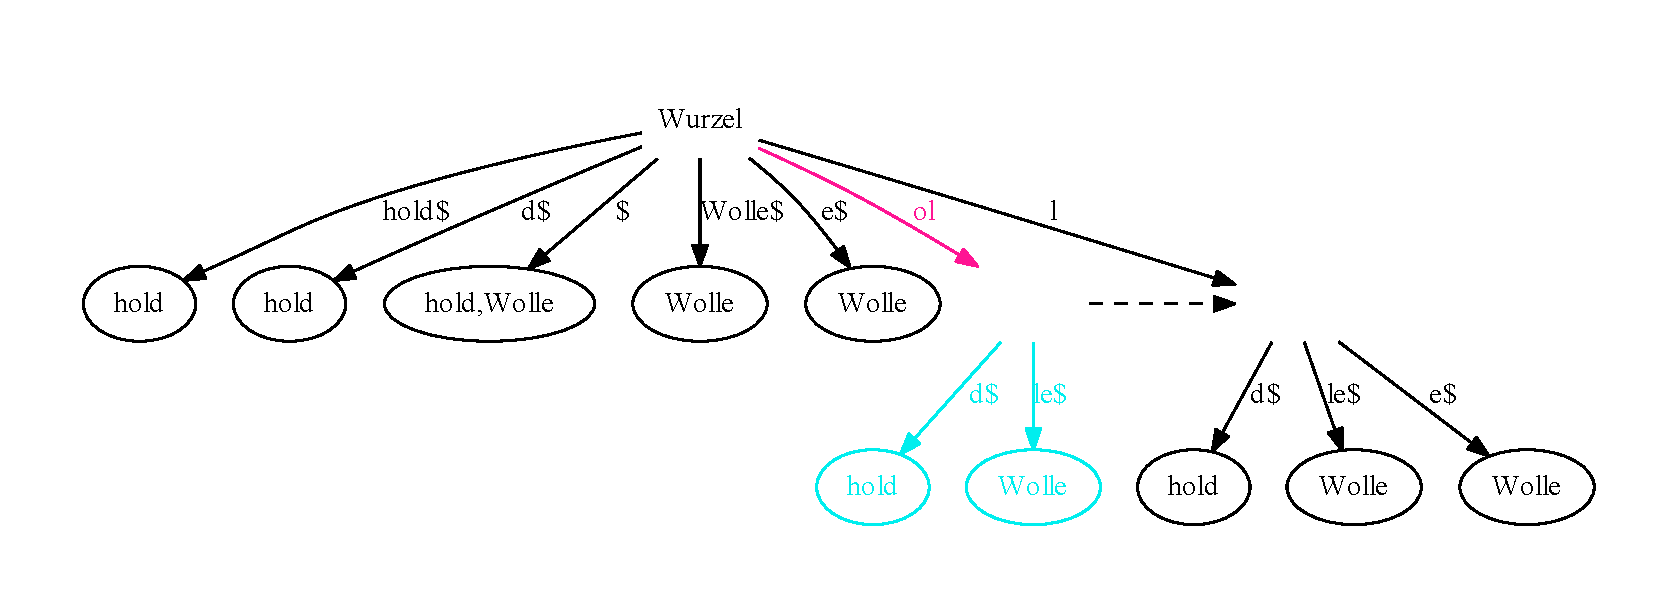
\includegraphics[scale=0.5]{resources/wolleHoldMatchSuffixTree.pdf}
\caption{Teilwortsuche für das Suchmuster \texttt{ol} in einem Beispiel-Suffixbaum für die Worte "`hold"' und "`Wolle"'. Bis zum Ende des pinken Bereichs konnte das Matching erfolgen. Die Suchergebnisse selbst müssen mit Tiefensuche aus dem Suffixbaum geholt werden (in türkis dargestellt).}
\label{fig-matchingSuffixTree}
\end{figure}

\newpage

\subsection{Einfache reguläre Ausdrücke}
\label{algo-regex}

\paragraph{} Wie in Kapitel \ref{algo-pattern-language} bereits angemerkt, wurde für \textit{BiBiServSearch} nur ein eingeschränkter Satz regulärer Ausdrücke implementiert. Dabei war das wesentliche Kriterium bei der Auswahl, dass alle Ausdrücke (bis auf \texttt{*}) je \textit{genau ein} Zeichen matchen. Diese Einschränkung bedeutet zwar eine echte Reduzierung des Funktionsumfangs, ermöglicht aber die Einteilung des Suchmusters in einzelne "`semantische Zeichen"' und vereinfacht dadurch Kompilierung und Suche (siehe auch \ref{arch-pattern}). Daher sind die sonst üblichen Oder-Ausdrücke hier nicht erlaubt (wie z.B. \texttt{(a|ab|abc)}, was bedeuten soll: Entweder $a$ oder $ab$ oder $abc$).
\paragraph{} Der Suchvorgang für reguläre Ausdrücke läuft in folgenden Schritten ab:

\begin{enumerate}
\item Umwandeln des Suchmuster-Strings in einen NEA (siehe auch \ref{meth-automata}).
\item Matching des Automaten gegen den generalisierten Suffixbaum.
\end{enumerate}

\subsubsection{Kompilierung des Suchmusters}

\paragraph{} Wie in Kapitel \ref{arch-pattern} beschrieben geschieht die Kompilierung des Suchmusters mittels eines Transduktors. Dabei wird jedes semantische Zeichen des Suchausdrucks jeweils genau einmal behandelt. Ein semantisches Zeichen eines regulären Ausdrucks kann eine von vier Kategorien haben:
\begin{itemize}
\item Es ist genau ein Zeichen erlaubt (\texttt{ExactPatternChar}), Beispiel: \texttt{a}
\item Es ist irgendein Element aus einer Menge von Zeichen erlaubt \\(\texttt{OneOfPatternChar}), Beispiel: \texttt{[xy]}
\item Es ist irgendein Zeichen erlaubt, das nicht in einer definierten Menge von Zeichen liegt (\texttt{NotOneOfPatternChar}), Beispiel: \texttt{[\^{ }xy]}
\item Es ist irgendein Zeichen erlaubt (\texttt{AnyPatternChar}), Beispiel: \texttt{.}
\end{itemize}
\paragraph{} Unterschieden wird zudem, ob das semantische Zeichen jeweils beliebig oft vorkommen darf oder nicht (ob also ein \texttt{*} folgt oder nicht). Der Kompilierungsalgorithmus ist im Detail als Pseudocode-Algorithmus \ref{code-pattern-compiling} beschrieben.

\begin{algorithm}
\caption{Kompilierung eines Suchmusters}
\label{code-pattern-compiling}
\begin{algorithmic}
\STATE{Initialisiere den momentanen Zustand $z_1$ mit einem leeren Startzustand.}
\STATE{Initialisiere den Stapel $S$ für semantische Zeichen, denen ein \texttt{*} folgt.}
\FORALL{semantische Zeichen $p_1$ des Suchmusters}
	\IF{Auf $p_1$ folgt ein \texttt{*}}
		\IF{Es wurde bereits ein semantisches Zeichen gelesen, dem kein \texttt{*} folgt}
			\STATE{Lege $p_1$ auf $S$.}
		\ENDIF
	\ELSE
		\STATE{Erzeuge einen neuen Zustand $z_2$ des endlichen Automaten.}
		\STATE{Erzeuge eine Kante von $z_1$ nach $z_2$, die mit $p_1$ beschrieben ist.}
		\IF{$S$ ist nicht leer}
			\STATE{Initialisiere die Menge $Z$ als eine Menge von Folgezuständen und Beschriftungen von Kanten, die zu ihnen führen.}
			\STATE{Lege das Tupel $(p_1,z_2)$ in $Z$.}
			\WHILE{$S$ ist nicht leer}
				\STATE{Nimm das oberste semantische Zeichen $p_2$ von $S$ herunter.}
				\IF{$S$ ist leer}
					\STATE{Setze $z_3$ $=$ $z_1$.}
				\ELSE
					\STATE{Erzeuge einen neuen Zustand $z_3$.}
				\ENDIF
				\STATE{Erzeuge eine Kante von $z_3$ nach $z_3$, die mit $p_2$ beschrieben ist.}
				\FORALL{Tupel $(p_3,z_4) \in Z$}
					\STATE{Erzeuge eine Kante von $z_3$ nach $z_4$, die mit $p_3$ beschrieben ist.}
				\ENDFOR
				\STATE{Lege das Tupel $(p_2,z_3)$ in $Z$.}
			\ENDWHILE
		\ENDIF
		\STATE{setze $z_1$ $=$ $z_2$.}
	\ENDIF
\ENDFOR
\STATE{Erzeuge einen akzeptierenden Zustand $f$.}
\STATE{Erzeuge eine Kante von $z_1$ nach $f$, die mit einem Endsymbol beschrieben ist.}
\end{algorithmic}
\end{algorithm}

\paragraph{} Dabei ist folgendes zu beachten:

\begin{itemize}
 \item Im Falle eines Suchmusters ohne reguläre Ausdrücke läuft dieser Algorithmus ohne Besonderheiten durch und betrachtet jedes Zeichen als \\\texttt{ExactPatternChar}.
 \item Für Zeichen, denen ein \texttt{*} folgt, wird ein Stapel/Stack angelegt. Bei der Abarbeitung des Stapels werden für alle Zeichen auf dem Stapel (bis auf das erste) neue Zustände angelegt. Für jeden dieser neuen Zustände müssen Kanten zu jeweils allen noch folgenden Zuständen gezogen werden, weil für jeden \texttt{*}-Ausdruck auch das leere Wort als Match erlaubt ist.
 \item Obwohl das im Pseudocode nicht benannt ist, werden für den Inhalt des Stapels noch Optimierungen durchgeführt: Optimierungen sind möglich, wenn von zwei benachbarten \texttt{*}-Ausdrücken A und B die von A definierte Sprache eine Teilmenge der Sprache von B ist oder umgekehrt (siehe auch \ref{arch-pattern}). Ein Beispiel dafür ist der Ausdruck \texttt{a*.*}. Dieser Ausdruck kann zu \texttt{.*} optimiert werden, weil $\lbrace a\rbrace$ eine Teilmenge des Gesamtalphabets ist.
 \item Da eine Teilwortsuche durchgeführt wird, steht am Beginn und Ende des Musters implizit ein \texttt{.*}. Aus diesem Grunde werden Zeichen, denen zwar ein \texttt{*} folgt, die aber am Beginn oder Ende des Musters stehen, einfach ignoriert.
\end{itemize}

\paragraph{} Das Ergebnis eines Kompilierungsprozesses ist in Abbildung \ref{fig-nea} an einem Beispiel illustriert.

\begin{figure}
\centering
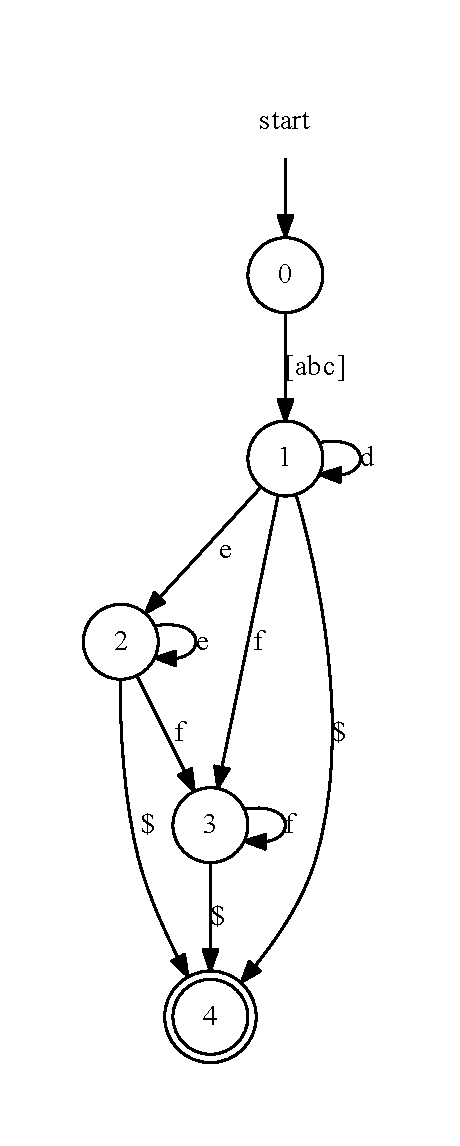
\includegraphics[scale=0.7]{resources/nea.pdf}
\caption{Ein NEA, der dem Suchmuster \texttt{[abc]d*e*f*} entspricht. Der Zustand mit dem "`start"'-Pfeil ist der Startzustand. Der Endzustand ist doppelt umkreist. Das "`\$"'-Zeichen ist ein Endsymbol.}
\label{fig-nea}
\end{figure}

\subsubsection{Matching}

\paragraph{} Der Matchingprozss wird nun über eine Art "`Meta-Automat"' aus dem NEA des Suchmusters und dem Suffixbaum erledigt. Die Zustände des Meta-Automa\-ten sind über die momentane Position im Suffixbaum und den Zustand im NEA charakterisiert. Nur wenn die Kombination aus beidem gleich ist, ist auch das Verhalten des Automaten gleich. Dabei ist zu beachten, dass der Matchingvorgang nicht mehr linear ist sondern indeterministisch mehrere Stränge des Matchings existieren, die über einen Stack künstlich nacheinander ausgeführt werden. Eine Parallelisierung der Ausführungspfade über Threading wäre hier grundsätzlich möglich, ist aber nicht implementiert.
\paragraph{} Diese Vorgehensweise ist analog zur Technik von Baeza-Yates und Gonnet (siehe \cite{baeza-yates}), allerdings in vereinfachter Form, weil hier zu Gunsten einer Beschleunigung der Suchmusterkompilierung NEAs und nicht DEAs implementiert wurden. Auch die bei Baeza-Yates und Gonnet vorgeschlagene binäre Kodierung des Suffixbaums ist hier nicht umgesetzt.
\paragraph{} Das Matching ist im Pseudocode-Algorithmus \ref{code-matching} beschrieben. Wie schon beschrieben kann dann für die Menge der Wort-IDs eine Menge von Vorkommen über den Hauptindex ermittelt werden.

\begin{algorithm}
\caption{Matching-Algorithmus}
\label{code-matching}
\begin{algorithmic}
\STATE{Initialisiere den Stapel der Zustände $S$ und lege den Initialzustand darauf (Wurzel des Baumes und Startzustand des NEA).}
\STATE{Initialisiere die Menge mit Ergebnis-Wort-IDs $W$.}
\WHILE{$S$ ist nicht leer}
	\STATE{Nimm den obersten Zustand $z$ von $S$ herunter.}
	\FORALL{ausgehende Kanten $p$ des NEA-Zustandes in $z$}
		\IF{$p$ ist Endsymbol}
			\STATE{Lege die IDs aller Worte in $W$, die an Blättern notiert sind, die bei einer Tiefensuche im Suffixbaum vom jetzigen Punkt aus zu finden sind.}
		\ELSE
			\IF{momentane Position im Baum ist eine Kante}
				\STATE{Sei $c$ das momentane Zeichen auf der Kante im Baum.}
				\IF{$c$ liegt in der Sprache von $p$}
					\STATE{Erzeuge einen neuen Zustand $z'$ mit der um 1 vorgerückten Baumposition und dem nächsten NEA-Zustand für $p$.}
					\STATE{Lege $z'$ auf $S$.}
				\ENDIF
			\ELSE
				\FORALL{ausgehende Kanten $c$ des momentanen Knotens im Baum, die in der Sprache von $p$ liegen}
					\STATE{Erzeuge einen neuen Zustand $z'$ mit der um 1 vorgerückten Baumposition auf Kante $e$ und dem nächsten NEA-Zustand für $p$.}
					\STATE{Lege $z'$ auf $S$.}
				\ENDFOR
			\ENDIF
		\ENDIF
	\ENDFOR
\ENDWHILE
\end{algorithmic}
\end{algorithm}

\subsection{Inexakte Suche}
\label{algo-inexact}

\paragraph{} Die inexakte Suche ist der komplexeste implementierte Suchmodus. Hier geht es darum, mit heuristischen Mitteln mögliche Tippfehler in Suchanfragen zu korrigieren. Zu diesem Zweck sollen auch \textit{hinreichend ähnliche} Worte als Matches für das Suchmuster zugelassen werden. Wie dieses \textit{hinreichend ähnlich} zu definieren ist steht dabei im Kern des folgenden Abschnitts. Danach wird die Umsetzung dieses Konzeptes besprochen.

\subsubsection{Konzept}

\paragraph{} Ein gängiges heuristisches Modell für die Behandlung von Tippfehlern ist die Betrachtung von Edit-Distanzen, wie sie von Damerau eingeführt wurde (siehe \cite{damerau}, S. 172 und \cite{jurafsky&martin}, S. 145). Die Edit-Distanz beschreibt die Zahl der Arbeitsschritte, die nötig ist, um ein Wort in ein anderes zu überführen. Als ein Arbeitsschritt gilt dabei:

\paragraph{}

\begin{tabularx}{\textwidth}{lX}
\hline
\textbf{Bezeichnung} & \textbf{Beschreibung und Beispiel} \\ [0.1cm]
\hline
insertion &  Weglassen eines Zeichens im Wort (aus "`hold"' wird z.B. "`old"') \\ [0.1cm]
\hline
deletion &  Einfügen eines Zeichens im Wort (aus "`hold"' wird z.B. "`holde"') \\ [0.1cm]
\hline
substitution & Ersetzen eines Zeichens im Wort (aus "`hold"' wird z.B. "`gold"') \\ [0.1cm]
\hline
transposition & Umtausch zweier Zeichen im Wort (aus "`hold"' wird z.B. "`hlod"') \\ [0.1cm]
\hline
\end{tabularx}

\paragraph{} Nach einer Studie von Peterson (siehe \cite{peterson}, S.634) sind etwa 93-94 \% der Tippfehler nur einen Arbeitsschritt vom eigentlich gemeinten Wort entfernt. Daher konzentriert sich die inexakte Suche hier darauf, genau diese Fehler mit Edit-Distanz 1 zu beheben.
\paragraph{} Die Idee ist dabei wie folgt: Versuche, das Suchwort wie in den vorherigen Kapiteln im Baum zu finden (siehe vor allem \ref{algo-regex}). Sobald ein Buchstabe im Suchwort nicht mehr mit dem Buchstaben im Baum übereinstimmt, versuche den Fehler zu beheben, in dem, falls möglich, jeder der obigen Arbeitsschritte angewendet wird. Bei einem erneuten Fehler wird der Suchvorgang abgebrochen.
\paragraph{} Dieser Algorithmus verzichtet dabei auf die Ansätze des dynamic programming, wie es bei Cobbs, Ukkonen und Jokinen Anwendung findet (siehe \cite{approxTreesUkkonen1, approxTreesUkkonen2,approxTreesCobbs}). Diese Vereinfachung ist nur deshalb zulässig, weil die maximale Edit-Distanz in der vorliegenden Implementierung 1 beträgt. Andernfalls könnte es passieren, dass durch mehrfache Anwendung von Edit-Operationen Zustände wiederholt werden und dadurch eine erheblich schlechtere worst-case-Laufzeit erzielt wird. Wegen der Vereinfachung ist es auch nicht nötig, eine von den o.g. Autoren vorgeschlagene Tabelle mit Edit-Operationen explizit aufzubauen. Diese wird mithin implizit über die \texttt{MatchingStates} kodiert.

\subsubsection{Umsetzung}

\paragraph{} Dass \textit{alle} Arbeitsschritte zur Fehlerkorrektur angewendet werden bedeutet, dass der Matchingvorgang indeterministisch wird. Da das bestehende System mit \texttt{MatchingStates} für reguläre Ausdrücke aber bereits in der Lage ist, Indeterminismus zu behandeln, liegt es nahe, einfach dieses System zu erweitern.
\paragraph{} Ein Zustand des dort besprochenen "`Meta-Automaten"' erhält also ein weiteres Charakteristikum: Ist die Anwendung eines Arbeitsschrittes noch erlaubt oder nicht (Bei einer Teilwortsuche, die kein inexaktes Matching erlaubt, wird dies schon im Initialzustand auf "`nein"' gesetzt)? Beim ersten mismatch wird versucht, den Fehler durch die Anwendung der beschriebenen Arbeitsschritte zu beheben. Beim neu entstehenden Zustand wird dann die Frage, ob die Anwendung eines Arbeitsschrittes erlaubt ist, mit "`nein"' beantwortet. So wird erreicht, dass alle Fehler mit einer Edit-Distanz von 1 behoben werden. Dank des Konzeptes des Meta-Automaten geschieht dies aber nur, wenn auch wirklich ein mismatch auftritt. Gegenüber der naiven Implementierung, einfach blind alle Permutationen des Suchmusters mit Edit-Distanz 1 zu erzeugen (klassische "`Neighborhood generation"' wie in \cite{approximateIndexing} beschrieben) und danach jeweils zu suchen, ist dieses Vorgehen also eine deutliche Verbesserung.
\paragraph{} Der für die Arbeitsschritte jeweils neue Zustand des Meta-Automaten wird wie folgt berechnet:

\paragraph{}

\begin{tabularx}{\textwidth}{lX}
\hline
\textbf{Bezeichnung} & \textbf{Neuer Zustand} \\ [0.1cm]
\hline
insertion & Rücke im Suffixbaum um einen Schritt vor. \\ [0.1cm]
\hline
deletion & Rücke im NEA zum nächsten Zustand vor. \\ [0.1cm]
\hline
substitution & Rücke sowohl im Suffixbaum als auch im NEA um einen Schritt vor. \\ [0.1cm]
\hline
transposition & Siehe unten. \\ [0.1cm]
\hline
\end{tabularx}

\paragraph{} Diese Operationen sind bis auf transpositions trivial umsetzbar. Transpositions werden wie in Algorithmus \ref{code-swap} beschrieben behandelt.

\begin{algorithm}
\caption{Transposition-Algorithmus}
\label{code-swap}
\begin{algorithmic}
\STATE{Sei $c$ das momentane Zeichen im Suffixbaum und $z_0$ der momentane Zustand des NEA.}
\FORALL{ausgehende Kanten $p_0$ von $z_0$}
\STATE{Sei $z_1$ der Folgezustand für $p_0$.}
\IF{$z_1$ $\neq$ $z_0$}
\FORALL{ausgehende Kanten $p_1$ von $z_1$, die $c$ akzeptieren}
\STATE{Sei $z_2$ der Folgezustand für $p_1$.}
\STATE{Erzeuge einen neuen NEA-Zustand $z_3$.}
\STATE{Erzeuge eine Kante von $z_3$ über $p_1$ nach $z_2$.}
\STATE{Setze $z_3$ als neuen NEA-Zustand. Die Position im Suffixbaum bleibt unverändert.}
\ENDFOR
\ENDIF
\ENDFOR
\end{algorithmic}
\end{algorithm}

\paragraph{} Über die Erzeugung des virtuellen NEA-Zustandes $z_3$ wird sicher gestellt, dass der NEA genau dann in den Zustand $z_2$ übergeht, wenn zwei Zeichen im Suchwort in genau umgekehrter Reihenfolge im Baum vorkommen. Das entspricht exakt dem, was man mit einer transposition erreichen wollte.
\paragraph{} Zudem ist über diesen Mechanismus das inexakte Matching mit regulären Ausdrücken kompatibel\footnote{Allerdings wird verhindert, dass \texttt{*}-Ausdrücke bei der Fehlerbehebung in Betracht gezogen werden. Edit-Operationen auf diesen Ausdrücken würden beispielsweise dazu führen, dass bei Anwendung der deletion-Regel im NEA auf den gleichen Zustand vorgerückt wird, sich also am Zustand eigentlich nichts ändert, das System aber trotzdem damit umgeht als sei hier eine Edit-Operation angewandt worden. Das könnte zu verwirrenden Ergebnissen für Nutzende führen.}.

\subsection{Bewertung der Suchergebnisse}
\label{algo-scoring}

\paragraph{} Nachdem eine Menge von Vorkommen der Ergebnisworte erstellt worden ist, ist der letzte Schritt die Umsetzung dieser Menge von Vorkommen in eine sortierte Liste von Dokumenten-Identifikatoren (siehe auch \ref{arch-docIndex}), die Nutzenden auf ihre jeweilige Suchanfrage hin zurückgegeben werden kann.
\paragraph{} Wie im Konzept vorgeschlagen (siehe \ref{meth-scoring}) erfolgt die Sortierung der Dokumente nach einem zweistufigen \texttt{SearchScore}:
\begin{enumerate}
\item Wie viele Vorkommen von Matches enthält das Dokument? (primärer Score)
\item Wie weit sind die Matches vom ursprünglichen Suchmuster entfernt? (sekundärer Score)
\end{enumerate}

\paragraph{} Dabei wird vornehmlich nach dem primären Score sortiert und erst bei gleichem Wert der sekundäre Score in Betracht gezogen. Das heißt: Dokumente, die mehr Treffer enthalten, werden auch als erstes genannt. Dokumente, die gleich viele Treffer enthalten, werden dann zuerst genannt, wenn die Treffer im Durchschnitt besser dem Suchmuster entsprechen.
\paragraph{} Der Prozess ist im Pseudocode-Algorithmus \ref{code-scoring} beschrieben.

\begin{algorithm}
\caption{Bewertungsalgorithmus für Suchergebnisse}
\label{code-scoring}
\begin{algorithmic}
\STATE{Initialisiere eine HashMap $H$, die Dokumente auf ihren \texttt{SearchScore} abbildet.}
\FORALL{Vorkommen $v$ in der Menge der Ergebnisvorkommen}
	\STATE{Sei $d$ das Dokument, das $v$ enthält.}
	\IF{$d$ ist in $H$ enthalten}
		\STATE{Sei $S$ das Score-Objekt für $d$.}
		\STATE{Erhöhe den Primärscore in $S$ um 1.}
		\STATE{Berechne den Sekundärscore $s'$ für v.}
		\STATE{Erhöhe den Sekundärscore in $S$ um $s'$.}
	\ELSE
		\STATE{Erstelle ein neues Score-Objekt $S$.}
		\STATE{Setze den Primärscore auf 1.}
		\STATE{Berechne den Sekundärscore $s'$ für v.}
		\STATE{Setze den Sekundärscore in $S$ auf $s'$}
	\ENDIF
	\STATE{Schreibe $S$ für $d$ in $H$.}
\ENDFOR
\end{algorithmic}
\end{algorithm}

\paragraph{} Die Berechnung des Sekundärscores unterscheidet sich dabei je nach Suchmodus. Generell gilt: Ein höherer Sekundärscore bedeutet eine größere Entfernung vom Suchmuster. Bei exakter Suche ist dieser Score immer 0 (weil ja \textit{per definitionem} Matches dem Suchmuster exakt entsprechen müssen). Bei der Teilwortsuche wird die Länge des Matches mit der Länge des gematchten Teilwortes verglichen. Die Differenz beider Längen ist der Sekundärscore. Bei der inexakten Suche erfolgt die Berechnung auf die gleiche Weise, es wird aber noch der Wert 3 addiert, falls Methoden der inexakten Suche benutzt werden mussten, um dieses Match zu finden.

\paragraph{} Zusätzlich wird für jedes Ergebnisvorkommen der \textit{Kontext} bestimmt, das heißt: Ausgehend vom Wort, das gematcht wurde, werden die vorherigen drei Worte und die nachfolgenden drei Worte bestimmt, um Nutzenden des Programms mehr Komfort zu bieten. Dies ist über die Referenzierung von Vorgängern und Nachfolgern bei Vorkommen möglich (siehe auch \ref{arch-index}).

\newpage

\subsection{Entfernen eines Dokuments}
\label{algo-removeDoc}

\paragraph{} Wenn ein Dokument aus dem Suchraum entfernt werden soll, wird das Dokument und sein Inhalt aus allen Indizes entfernt. Zuerst wird für eine gegebene URL die Dokumenten-ID aus dem Dokumentenindex herausgesucht. Mit dieser ID kann über den Hauptindex iteriert und es können alle Vorkommen entfernt werden, die auf diese ID verweisen. Zusätzlich wird bei dieser Gelegenheit auch geprüft, ob die Menge von Vorkommen, auf die eine Wort-ID im Hauptindex verweist, leer geworden ist. Falls ja wird der Eintrag dieses Wortes ganz aus Haupt- und Wortindex entfernt.
\paragraph{} Problematisch dabei ist, dass die Worte nicht aus dem Suffixbaum entfernt werden können (siehe auch \ref{meth-addAndRemove}). Auf die Suchergebnisse hat das keinen Einfluss, denn im Hauptindex wird dann für die fragliche Wort-ID schlicht kein Verweis auf die gelöschten Dokumente gefunden. Dennoch führt das langfristig dazu, dass der Suffixbaum mit Einträgen, die zu keinem Ergebnis mehr führen, überfüllt wird. Das kostet Speicher und Rechenzeit beim Suchen.
\paragraph{} Wie im Konzept beschrieben (siehe \ref{meth-addAndRemove}), wurden zwei Mechanismen eingeführt, um dieses Problem zu entschärfen:
\begin{enumerate}
 \item Von außen kann bei Bedarf die Funktion \texttt{rebuildTree} der Klasse \texttt{WordIndex} aufgerufen werden. Bei einem Aufruf wird der Suffixbaum neu aus dem momentanen Wortindex aufgebaut. Dabei werden  gelöschte Einträge nicht mehr mit in den neuen Baum übernommen und der alte Baum wird aus dem Speicher gelöscht.
 \item Beim Neueinfügen von Dokumenten in den Baum wird der Baum ebenfalls neu aufgebaut (siehe auch \ref{arch-session}). Auch dabei werden alle gelöschten Einträge nicht mehr in den neuen Baum übernommen.
\end{enumerate}